\chapter{Measuring samples}
\index{Sample!Measuring|(}
Although it is possible to manually enter the ring widths of your samples into Corina, it is normal to automate this process using a measuring platform. Corina supports the most common measuring platforms including Velmex and Lintab.  For details on how to configure your measuring platform see section \ref{txt:MeasuringPlatformConfig}.

Once your measuring platform has been configured, measuring your first sample is simple.  To start a new measurement go to \menutwo{File}{New} or click the `new' icon on the home screen. A dialog will appear where you can scan your sample's barcode, or press the button to enter metadata for your sample later. Barcodes minimize data entry errors and also speed up the process of measuring your samples. See section \ref{txt:barcode} for more information. Once you have scanned your barcode or pressed the button, you will then be presented with an empty Corina data screen (figure \ref{fig:datascreen}).

\begin{figure}[hbtp]
  \centering
    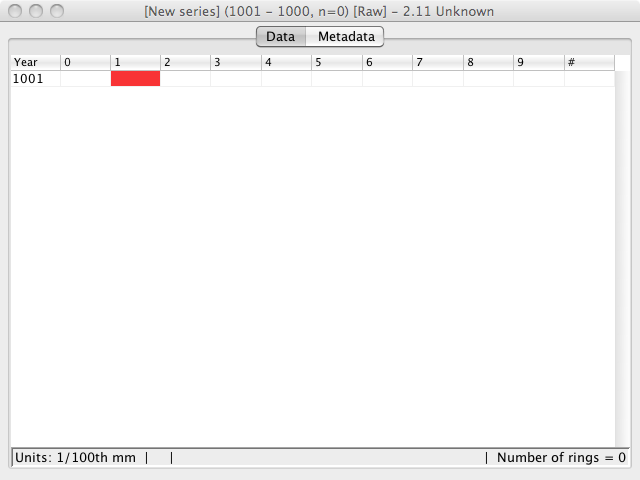
\includegraphics[width=0.6\textwidth]{Images/datascreen.png}
    \caption{An empty data window ready to receive measurements.  Note the status bar at the bottom includes buttons for changing the display units and cumulative statistics.}
    \label{fig:datascreen}
\end{figure}

The next step is to fill out the metadata tab. If you have used a barcode, nearly all of this metadata will be filled in for you, otherwise you will need to fill this out yourself. Details about metadata can be found in chapter \ref{txt:metadata}, page \pageref{txt:metadata}.

To begin measuring your sample you can now go to \menutwo{Edit}{Start measuring} or you can press F5. Depending on the type of platform you have you will have different buttons available at the bottom of the screen.  If you platform accepts requests for measurement data, or accepts requests to zero the measurement then you will have buttons available to do so.  Otherwise you will need to use the hardware buttons on your device to send measurements to Corina.

While measuring you should be provided with audible feedback for each ring measured with a more pronounced sound made every 10th ring. If there is a problem communicating with your measuring hardware, check your settings in the preferences dialog. If you still have problems contact the Corina developers by going to \menutwo{Help}{Report bug on last transaction}, making sure you include your email address and any further relevant information.


\index{Ring remarks}
While you measure your sample you can flag features in a ring by right clicking on any cell in the table and selecting one or more of the standard notes (see figure \ref{fig:ringremarks}).

\begin{wrapfigure}{r}{0.5\textwidth}
  \begin{center}
    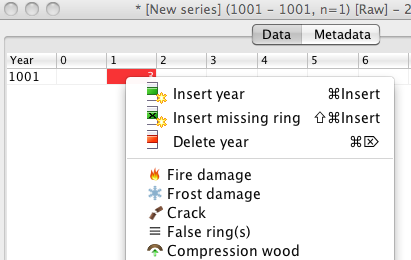
\includegraphics[width=0.48\textwidth]{Images/ringremarks.png}
  \end{center}
  \caption{Right click context menu showing some of the options for adding remarks to rings.}
  \label{fig:ringremarks}
\end{wrapfigure}

Corina supports all standard TRiDaS remarks including: fire damage; frost damage; crack; false ring(s); compression wood; tension wood; traumatic ducts; single pinned; double pinned; triple pinned and many others.  Rings that include remarks are indicated by the relevant icon in the data screen.  Depending on your method of work, this can be useful for keeping track of sample pin holes.  For instance, if a missing or false ring is discovered after a sample has been pinholed, the offset in pinholes can be easily seen without resurfacing the sample.  In the future Corina will also include support for user defined ring remarks.  

The data screen also contains a status bar at the bottom. By click on the units section, you can switch between micron and 1/100th mm units. Corina understands the units being supplied by the measuring platform, therefore changes here are purely for display purposes only. If you have a platform that measures in microns, but prefer to see the values in 1/100th mm then you can use this feature. At the bottom ring of the status bar you can choose one of a variety of summary information about your series.

Once you have finished measuring your sample, you should then go to \menutwo{File}{Save} to save your series to the database. 

\section{Reconciling data}
\index{Sample!Reconciling}
Corina has been developed not only for experience dendrochronologists, but as a tool for teaching students.  It therefore includes a comprehensive `reconciling' tool for supervisors to check the quality of measurements made by students.  The reconcile dialog does a comparison of a measurement series made by a student with a references series of the same radius measured by the supervisor.  The same dialog can also prove useful for comparing measurements from two experienced dendrochronologists when handling particularly difficult samples.

 

\index{Sample!Measuring|)}
